\section{DnsA}\label{sec:dnsa}

\begin{figure}
\begin{center}
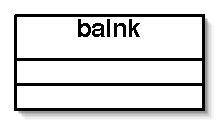
\includegraphics[width=0.4\textwidth]{figs/blank}
\end{center}
\caption{}
\label{fig:dnsa}
\end{figure}

This section describes the DnsA component, which is described by Figure~\ref{fig:dnsa}.  

The DnsA is a subclass of DnsRR which implements a common A resource record.

\subsection{Methods}

{\bf Public Methods}
\begin{itemize}
\item rdata\_valid(): Check if the data is valid
\item ip(): Get the IP
\item set\_ip(): Set the IP.
\end{itemize}

